\documentclass[conference]{IEEEtran}
\IEEEoverridecommandlockouts

\usepackage{cite}
\usepackage{amsmath,amssymb,amsfonts}
\usepackage{algorithmic}
\usepackage{graphicx}
\usepackage{textcomp}
\usepackage{xcolor}
\usepackage{booktabs}
\usepackage{array}
\usepackage{multirow}
\usepackage{url}

\def\BibTeX{{\rm B\kern-.05em{\sc i\kern-.025em b}\kern-.08em
    T\kern-.1667em\lower.7ex\hbox{E}\kern-.125emX}}

\begin{document}

\title{Comparative Analysis of Minimax with Alpha-Beta Pruning and MCTS-UCT for Tic-Tac-Toe}

\author{
\IEEEauthorblockN{Pham Thien Minh}
\IEEEauthorblockA{\textit{University of Engineering and Technology} \\
\textit{Vietnam National University, Hanoi (UET-VNU)}\\
Hanoi, Vietnam}
\and
\IEEEauthorblockN{Luc Gia Bao}
\IEEEauthorblockA{\textit{University of Engineering and Technology} \\
\textit{Vietnam National University, Hanoi (UET-VNU)}\\
Hanoi, Vietnam}
}

\IEEEaftertitletext{\vspace{-1.2\baselineskip}\begin{center}\textit{Note: Group member Nguyen Khac Trong is currently on temporary academic leave and did not participate in this project.}\end{center}\vspace{0.6\baselineskip}}

\maketitle

\begin{abstract}
We present an implementation and empirical comparison of two classical game-tree search algorithms---Minimax with Alpha-Beta pruning and Monte Carlo Tree Search with Upper Confidence Bound applied to Trees (MCTS-UCT)---on both classic $3\times 3$ Tic-Tac-Toe and $15\times 15$ five-in-a-row (Gomoku). Alpha-Beta pruning reduces the visited node count of Minimax by $71.8\%$ at depth $4$ on $3\times 3$ and by $88.0\%$ at depth $3$ on $15\times 15$ without altering the chosen move. On $3\times 3$ Tic-Tac-Toe, MCTS-UCT with $\ge 1000$ iterations achieves $0$ losses across $50$ alternating-first-move games against both a random agent and an optimal depth-$9$ Alpha-Beta opponent. Across exploration constants $c \in \{0.5, 1.0, 1.4, 2.0\}$, $c = 0.5$ converges fastest under tight budgets on $15\times 15$ ($100\%$ win rate at $200$ iterations), while $c \in \{1.0, 1.4\}$ reach $100\%$ ($50/50$) at $500$ iterations. Replacing random rollout with a lightweight one-step tactical heuristic rollout improves win rate by $+6.0\%$ on $3\times 3$ ($84.0\% \rightarrow 90.0\%$) and $+16.0\%$ on $15\times 15$ ($76.0\% \rightarrow 92.0\%$), illustrating the principle behind value and policy networks in modern systems such as AlphaGo. We also derive UCT from Multi-Armed Bandit regret bounds and explain why final move selection uses visit count $N$ rather than empirical win rate $W/N$.
\end{abstract}

\begin{IEEEkeywords}
Minimax, Alpha-Beta Pruning, Monte Carlo Tree Search, UCT, Multi-Armed Bandit, Tic-Tac-Toe, Gomoku
\end{IEEEkeywords}

\section{Introduction}
Game-tree search is a cornerstone of artificial intelligence research, with applications ranging from board games to automated planning and scheduling~\cite{russell2020}. Tic-Tac-Toe---despite its simple rules---serves as an ideal benchmark for comparing exact deterministic search (Minimax with Alpha-Beta pruning) and stochastic anytime search (MCTS-UCT), especially when scaled from $3\times 3$ (three-in-a-row) to $15\times 15$ (five-in-a-row / Gomoku), where exhaustive search becomes computationally intractable.

This study investigates five research questions:
\begin{itemize}
    \item \textbf{RQ1:} How much does Alpha-Beta pruning reduce the search tree compared to plain Minimax on $3\times 3$ and $15\times 15$ boards?
    \item \textbf{RQ2:} How does the UCT exploration constant $c \in \{0.5, 1.0, 1.4, 2.0\}$ affect win rate across iteration budgets?
    \item \textbf{RQ3:} Does MCTS-UCT never lose on $3\times 3$ Tic-Tac-Toe, and at what iteration threshold does this hold?
    \item \textbf{RQ4:} How much does a lightweight heuristic rollout improve MCTS over random rollout, and what is the runtime trade-off?
    \item \textbf{RQ5:} Why should the final move be selected by visit count $N$ rather than empirical win rate $W/N$?
    \item \textbf{RQ6 (Bonus):} How do UCT formula ablations (removing $\sqrt{\cdot}$, $\ln$, or both) and a Progressive Bias improvement affect search performance?
\end{itemize}

\section{Problem Formulation}
The game is modelled as a two-player, zero-sum, deterministic, perfect-information game:
\begin{itemize}
    \item \textbf{State $s$:} An $n \times n$ grid with cells in $\{X (+1), O (-1), \emptyset (0)\}$, where $X$ moves first.
    \item \textbf{Action $a$:} Placing the current player's marker on an empty cell. To keep search tractable on $15\times 15$, \texttt{get\_legal\_moves()} restricts candidates to empty cells within Chebyshev distance $\text{radius} = 2$ of existing stones (and forces the center cell $(\lfloor n/2 \rfloor, \lfloor n/2 \rfloor)$ on an empty board). Radius $2$ preserves one-gap tactical threats such as \texttt{\_ O \_ O \_}.
    \item \textbf{Terminal test:} $\text{win\_len}$ consecutive markers horizontally, vertically, or diagonally ($3$ on $3\times 3$; $5$ on $15\times 15$), or a full board (draw).
    \item \textbf{Utility:} For Minimax/Alpha-Beta, $+1{,}000{,}000$ (win), $-1{,}000{,}000$ (loss), $0$ (draw), or heuristic score $\text{eval}(s, p)$ at depth cutoff. For MCTS-UCT, $1.0$ (win), $0.5$ (draw or truncated rollout), and $0.0$ (loss), bounded in $[0, 1]$ as required by UCB1.
\end{itemize}

\section{Methods}

\subsection{Minimax with Alpha-Beta Pruning and Evaluation Function}
Minimax performs depth-first search up to $\text{max\_depth}$, assuming both players play optimally:
\begin{equation}
V(s, d) =
\begin{cases}
\text{eval}(s, \text{me}), & \text{if terminal}(s) \text{ or } d = 0 \\
\max_{a \in A(s)} V(s', d - 1), & \text{if MAX turn} \\
\min_{a \in A(s)} V(s', d - 1), & \text{if MIN turn}
\end{cases}
\end{equation}
where $s' = T(s, a)$ is the resulting state after action $a$.
Alpha-Beta maintains two bounds---$\alpha$ (best guaranteed score for MAX) and $\beta$ (best guaranteed score for MIN)---and prunes any subtree once $\alpha \ge \beta$. Under optimal move ordering, time complexity drops from $\mathcal{O}(b^d)$ to $\mathcal{O}(b^{d/2})$, effectively doubling searchable depth.

\textbf{Heuristic Evaluation Function (\texttt{evaluate}):} At non-terminal depth cutoffs, the board is scanned along all four directions (horizontal, vertical, main diagonal, anti-diagonal). For each contiguous run of length $L$ belonging to player $p$, empty spaces on both sides ($\text{space\_left}$, $\text{space\_right}$) are counted. If $L + \text{space\_left} + \text{space\_right} < \text{win\_len}$, the line cannot form a winning sequence and scores $0$. Otherwise, $\text{open\_ends} \in \{1, 2\}$ counts adjacent empty cells (capped at $1$ if total available space equals $\text{win\_len}$), and the pattern is scored non-linearly according to Table~\ref{tab:eval_weights}. The final heuristic value is $\text{total\_score}(\text{me}) - \text{total\_score}(\text{opponent})$. Exponential scaling forces Minimax to prioritize creating or blocking open fours over accumulating minor twos, while the $10\times$ multiplier for two open ends reflects that an opponent can only block one side per turn.

\begin{table}[t]
\centering
\caption{Pattern Weights in the Heuristic Evaluation Function}
\label{tab:eval_weights}
\begin{tabular}{@{}ccrl@{}}
\toprule
Length & Open Ends & Score & Tactical Meaning \\
\midrule
5 & 1 or 2 & 100,000 & Winning line \\
4 & 2 & 50,000 & Unstoppable double threat \\
4 & 1 & 5,000 & Immediate threat (blockable) \\
3 & 2 & 2,000 & Strong open three ($10\times$ single-open) \\
3 & 1 & 200 & Closed three \\
2 & 2 & 100 & Developing open two \\
2 & 1 & 10 & Closed two \\
1 & 2 / 1 & 5 / 1 & Minor positional bias \\
\bottomrule
\end{tabular}
\end{table}

\subsection{MCTS + UCT and Mathematical Foundation}
MCTS incrementally builds an asymmetric search tree over $K$ iterations of four phases~\cite{coulom2006,kocsis2006}:
\begin{enumerate}
    \item \textbf{Selection:} Starting at the root, descend via \texttt{best\_child(c)} maximizing UCT until reaching a node that is either terminal or not fully expanded.
    \item \textbf{Expansion:} Pop one untried legal move and attach a new child node.
    \item \textbf{Simulation (Rollout):} Play from the new node using \texttt{rollout\_fn} and obtain outcome $r \in \{0.0, 0.5, 1.0\}$ from the perspective of \texttt{node.player} (the player who just moved to reach \texttt{node}).
    \item \textbf{Backpropagation:} Walk up to the root, incrementing $N \leftarrow N + 1$, adding $W \leftarrow W + r$ (except at the root, which has no incoming move), and flipping perspective $r \leftarrow 1.0 - r$ at each parent step because parent and child represent opposing players.
\end{enumerate}

The UCT selection policy for child $i$ is:
\begin{equation}
\text{UCT}_i = \underbrace{\frac{W_i}{N_i}}_{\text{Exploitation}} + c\,\underbrace{\sqrt{\frac{\ln N_{\mathrm{parent}}}{N_i}}}_{\text{Exploration}}
\label{eq:uct}
\end{equation}
Unvisited children ($N_i = 0$) are assigned $+\infty$ so every legal move is tried at least once before UCT comparison begins.

\textbf{Mathematical Foundation (Multi-Armed Bandit \& UCB1):} At each internal node, choosing among $K$ legal moves is an instance of the stochastic Multi-Armed Bandit (MAB) problem: each child $i$ is an arm with unknown true expected reward $\mu_i \in [0, 1]$. Auer et al.~\cite{auer2002} introduced the UCB1 policy, which selects the arm maximizing the upper confidence bound of $\mu_i$.

The square-root and logarithmic terms arise directly from Hoeffding's inequality. For $N_i$ i.i.d.\ samples $X_1, \dots, X_{N_i} \in [0, 1]$ with empirical mean $\bar{X}_i = W_i / N_i$ and true mean $\mu_i$:
\begin{equation}
P(\bar{X}_i - \mu_i \ge \epsilon) \le e^{-2 N_i \epsilon^2}, \qquad
P(\mu_i - \bar{X}_i \ge \epsilon) \le e^{-2 N_i \epsilon^2}.
\end{equation}
Setting the tail probability bound to $N_{\mathrm{parent}}^{-4}$---the smallest integer exponent ensuring that summing over all $\le t^2$ visit-count pairs $(s, s_i)$ at step $t$ yields a convergent series $\sum_{t=1}^{\infty} t^2 \cdot t^{-4} = \sum_{t=1}^{\infty} t^{-2} = \pi^2/6 < \infty$ and keeps the residual error $\mathcal{O}(1)$---yields:
\begin{equation}
e^{-2 N_i \epsilon^2} = N_{\mathrm{parent}}^{-4} \implies \epsilon = \sqrt{\frac{2 \ln N_{\mathrm{parent}}}{N_i}}.
\end{equation}
Thus, with high probability, $\mu_i \le W_i/N_i + \sqrt{2 \ln N_{\mathrm{parent}} / N_i}$. Choosing the arm with the highest upper bound guarantees \emph{optimism in the face of uncertainty}: the $\ln N_{\mathrm{parent}}$ numerator grows sub-linearly so neglected arms are revisited infinitely often at a vanishing rate, while $1/\sqrt{N_i}$ shrinks the confidence interval as samples accumulate. Auer et al.~\cite{auer2002} proved that UCB1 achieves logarithmic cumulative regret:
\begin{equation}
R(N) \le \sum_{i:\,\Delta_i > 0} \frac{8 \ln N}{\Delta_i} + \mathcal{O}(1), \qquad \Delta_i = \mu^* - \mu_i,
\end{equation}
matching the Lai--Robbins asymptotic lower bound $\Omega(\ln N)$ up to constant factors. Kocsis and Szepesv\'ari~\cite{kocsis2006} extended UCB1 recursively to game trees (UCT), proving convergence to the minimax-optimal move as $N \to \infty$. In practice, the theoretical constant $\sqrt{2} \approx 1.414$ assumes stationary i.i.d.\ rewards in $[0, 1]$; in game trees, rollout rewards are non-stationary as deeper subtrees expand, motivating empirical tuning of $c$.

\subsection{Rollout Strategies}
\begin{itemize}
    \item \textbf{Random rollout (\texttt{random\_rollout}):} Selects uniformly random legal moves up to $\text{MAX\_ROLLOUT\_STEPS} = 30$ steps. On $3\times 3$, games finish within $\le 9$ moves so truncation never triggers. On $15\times 15$, random play rarely forms five-in-a-row within $30$ moves; truncated simulations return $0.5$ (undecided) to keep runtime bounded and avoid parity bias.
    \item \textbf{Heuristic rollout (\texttt{heuristic\_rollout}):} At each simulation step (also capped at $30$ steps), checks all legal moves in order: (1) play an immediate winning move if one exists; (2) otherwise block an opponent's immediate winning move; (3) otherwise pick uniformly at random. This one-ply tactical filter approximates a lightweight policy/value prior and is the conceptual precursor to the neural policy and value networks in AlphaGo~\cite{silver2016}.
\end{itemize}

\subsection{UCT Variants and Progressive Bias Improvement}
To empirically verify the necessity of both $\sqrt{\cdot}$ and $\ln$ in Eq.~\eqref{eq:uct} and improve low-budget search on $15\times 15$, we evaluate four ablations alongside an improved Progressive Bias formula~\cite{chaslot2008}:
\begin{itemize}
    \item \textbf{Standard UCT:} $W_i/N_i + c\sqrt{\ln N_{\mathrm{parent}} / N_i}$.
    \item \textbf{No-sqrt:} $W_i/N_i + c\,(\ln N_{\mathrm{parent}} / N_i)$.
    \item \textbf{No-ln:} $W_i/N_i + c\sqrt{N_{\mathrm{parent}} / N_i}$.
    \item \textbf{Linear:} $W_i/N_i + c\,(N_{\mathrm{parent}} / N_i)$.
    \item \textbf{Progressive Bias (Improved UCT):}
    \begin{equation}
    \text{UCT}_{\mathrm{PB}}(i) = \frac{W_i}{N_i} + c\sqrt{\frac{\ln N_{\mathrm{parent}}}{N_i}} + \frac{H_i}{N_i + 1},
    \end{equation}
    where $H_i = \frac{1}{2}\bigl(1 + \tanh(\text{eval}(s_i, p_i)/5000)\bigr) \in (0, 1)$ is cached once per node. As $N_i \to \infty$, $H_i/(N_i+1) \to 0$, preserving UCT's asymptotic optimality while guiding early exploration on large boards.
\end{itemize}

\section{Experimental Setup}
All experiments were executed in Python 3.14 (NumPy, Matplotlib) on a 12-core CPU using parallel game workers (\texttt{ProcessPoolExecutor}) with deterministic per-game seeds and alternating first-player assignment ($X$ on even games, $O$ on odd games) to eliminate first-move bias. Table~\ref{tab:setup} summarizes the experimental configurations.

\begin{table}[t]
\centering
\caption{Summary of Experimental Configurations}
\label{tab:setup}
\setlength{\tabcolsep}{3.5pt}
\begin{tabular}{@{}llll@{}}
\toprule
Experiment & Board & Opponent & Games \\
\midrule
Minimax vs AB & $3\times 3$, $15\times 15$ & Fixed states & 1 state \\
MCTS $c \times$ iters & $3\times 3$ & Random & 100 \\
MCTS $c \times$ iters & $15\times 15$ & Random & 50 \\
Never-lose check & $3\times 3$ & AB (d=9), Rand & 50 \\
Rollout compare & $3\times 3$ / $15\times 15$ & Random & 100 / 50 \\
UCT variants & $3\times 3$ / $15\times 15$ & AB (d=9), Rand & 100 / 50 \\
\bottomrule
\end{tabular}
\end{table}

\section{Results}

\subsection{Minimax vs Alpha-Beta: Node Count}
Table~\ref{tab:minimax_ab} and Figs.~\ref{fig:nodes_3x3}--\ref{fig:nodes_15x15} compare the number of visited nodes between plain Minimax and Alpha-Beta pruning. On $3\times 3$, Alpha-Beta reduces visited nodes by $71.8\%$ at depth $4$; on $15\times 15$, the reduction reaches $88.0\%$ at depth $3$ ($85{,}290 \rightarrow 10{,}257$ nodes).

\begin{table}[t]
\centering
\caption{Visited Nodes: Minimax vs Alpha-Beta Pruning}
\label{tab:minimax_ab}
\begin{tabular}{@{}ccrrr@{}}
\toprule
Board & Depth & Minimax Nodes & Alpha-Beta Nodes & Reduction \\
\midrule
$3\times 3$ & 1 & 7 & 7 & 0.0\% \\
$3\times 3$ & 2 & 49 & 32 & 34.7\% \\
$3\times 3$ & 3 & 259 & 132 & 49.0\% \\
$3\times 3$ & 4 & 979 & 276 & \textbf{71.8\%} \\
\midrule
$15\times 15$ & 1 & 36 & 36 & 0.0\% \\
$15\times 15$ & 2 & 1,634 & 410 & 74.9\% \\
$15\times 15$ & 3 & 85,290 & 10,257 & \textbf{88.0\%} \\
\bottomrule
\end{tabular}
\end{table}

\begin{figure}[t]
\centering
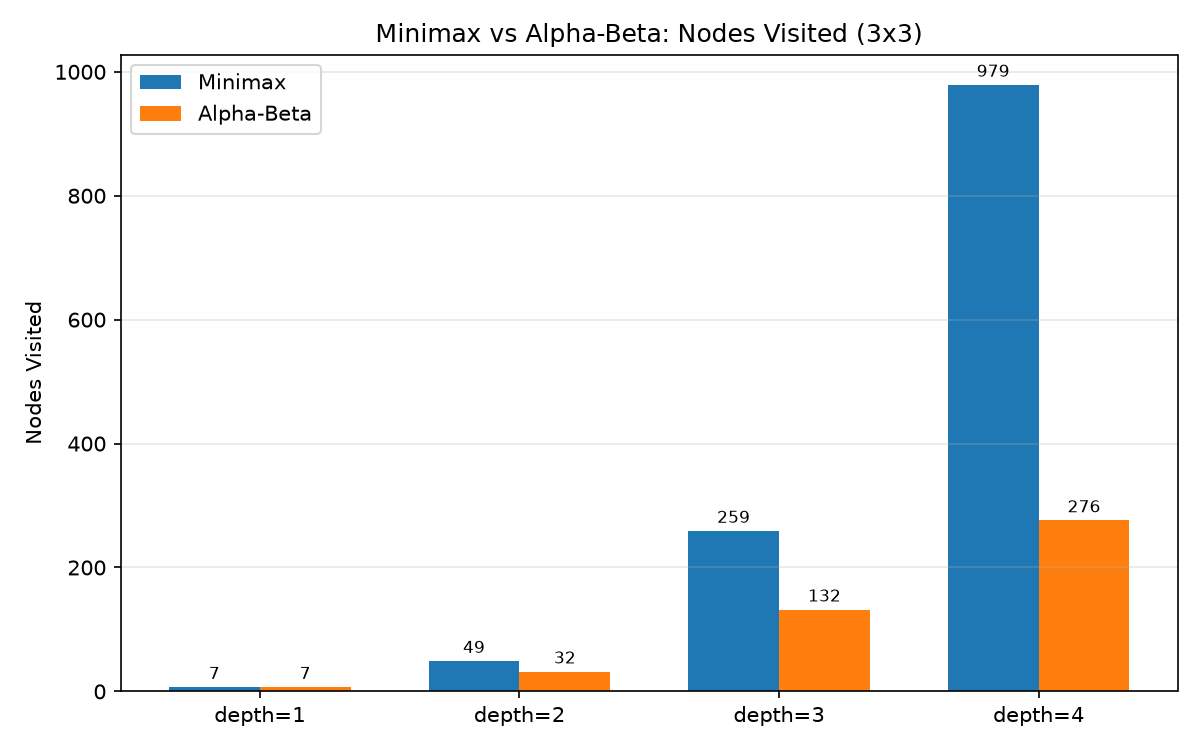
\includegraphics[width=0.95\linewidth]{../assets/figures/nodes_minimax_vs_ab_3x3.png}
\caption{Visited nodes comparison on the $3\times 3$ test state.}
\label{fig:nodes_3x3}
\end{figure}

\begin{figure}[t]
\centering
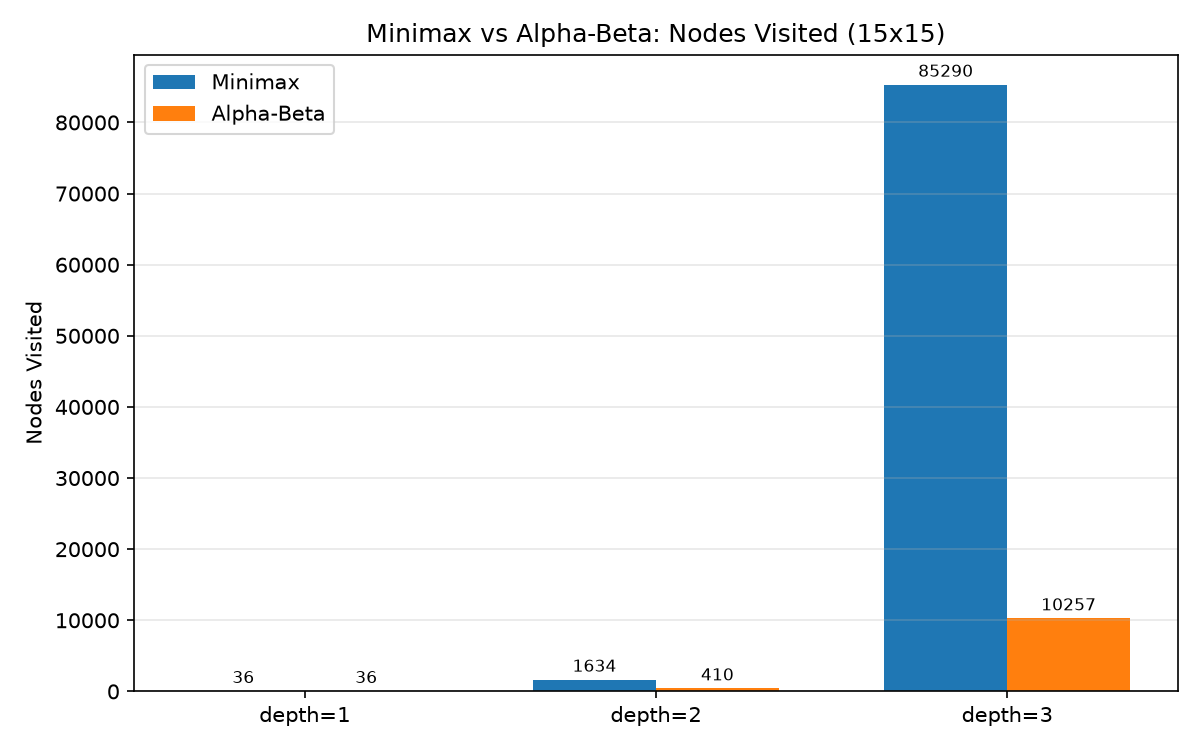
\includegraphics[width=0.95\linewidth]{../assets/figures/nodes_minimax_vs_ab_15x15.png}
\caption{Visited nodes comparison on the $15\times 15$ opening state.}
\label{fig:nodes_15x15}
\end{figure}

\subsection{MCTS Never-Lose Verification on $3\times 3$}
Table~\ref{tab:never_lose} reports MCTS-UCT outcomes against an optimal depth-$9$ Alpha-Beta opponent (which searches the entire $3\times 3$ game tree) and a random baseline across $50$ alternating games per configuration. At $100$ and $500$ iterations, MCTS still suffers occasional losses against optimal play ($11/50$ and $2/50$ for $c=1.0$). From $1000$ iterations onward, MCTS achieves \textbf{0 losses} ($50$ draws) against optimal Alpha-Beta and \textbf{0 losses} against random play from $500$ iterations onward.

\begin{table}[t]
\centering
\caption{MCTS-UCT Never-Lose Verification on $3\times 3$ (50 Games/Config)}
\label{tab:never_lose}
\begin{tabular}{@{}lcrrrr@{}}
\toprule
Opponent & $c$ & Iterations & Wins & Draws & Losses \\
\midrule
Alpha-Beta (d=9) & 1.0 & 100 & 0 & 39 & 11 \\
Alpha-Beta (d=9) & 1.0 & 500 & 0 & 48 & 2 \\
Alpha-Beta (d=9) & 1.0 & 1000 & 0 & 50 & \textbf{0} \\
Alpha-Beta (d=9) & 1.0 & 2000 & 0 & 50 & \textbf{0} \\
Alpha-Beta (d=9) & 1.414 & 100 & 0 & 41 & 9 \\
Alpha-Beta (d=9) & 1.414 & 500 & 0 & 48 & 2 \\
Alpha-Beta (d=9) & 1.414 & 1000 & 0 & 50 & \textbf{0} \\
Alpha-Beta (d=9) & 1.414 & 2000 & 0 & 50 & \textbf{0} \\
\midrule
Random & 1.0 & 100 & 46 & 2 & 2 \\
Random & 1.0 & 500 & 41 & 9 & \textbf{0} \\
Random & 1.0 & 1000 & 40 & 10 & \textbf{0} \\
Random & 1.0 & 2000 & 44 & 6 & \textbf{0} \\
Random & 1.414 & 100 & 44 & 2 & 4 \\
Random & 1.414 & 500 & 41 & 9 & \textbf{0} \\
Random & 1.414 & 1000 & 41 & 9 & \textbf{0} \\
Random & 1.414 & 2000 & 44 & 6 & \textbf{0} \\
\bottomrule
\end{tabular}
\end{table}

\subsection{Win Rate vs Iterations ($3\times 3$ and $15\times 15$)}
Tables~\ref{tab:mcts_3x3}--\ref{tab:mcts_15x15} and Figs.~\ref{fig:winrate_3x3}--\ref{fig:winrate_15x15} show MCTS win rates against a random agent across $c \in \{0.5, 1.0, 1.4, 2.0\}$. On $3\times 3$, all four constants reach $0$ losses once $\text{iterations} \ge 500$, plateauing at $84$--$90\%$ win rate (remaining games are draws when playing second). On $15\times 15$, $c = 0.5$ converges fastest at low budgets ($64.0\%$ at $100$ iterations, $100.0\%$ at $200$ iterations), whereas at $500$ iterations $c = 1.0$ and $c = 1.4$ both achieve $100.0\%$ ($50/50$).

\begin{table}[t]
\centering
\caption{MCTS Win Rate (\%) on $3\times 3$ (100 Games/Config, W/D/L)}
\label{tab:mcts_3x3}
\setlength{\tabcolsep}{3.5pt}
\begin{tabular}{@{}rcccccc@{}}
\toprule
$c$ & 50 & 100 & 200 & 500 & 1000 & 2000 \\
\midrule
0.5 & 82.0 & 81.0 & 91.0 & 89.0 & 87.0 & 87.0 \\
1.0 & 81.0 & 81.0 & 88.0 & 87.0 & 88.0 & 88.0 \\
1.4 & 87.0 & 90.0 & 84.0 & 86.0 & 84.0 & 90.0 \\
2.0 & 87.0 & 83.0 & 86.0 & 90.0 & 85.0 & 82.0 \\
\bottomrule
\end{tabular}
\end{table}

\begin{table}[t]
\centering
\caption{MCTS Win Rate (\%) on $15\times 15$ (50 Games/Config, W/D/L)}
\label{tab:mcts_15x15}
\begin{tabular}{@{}rcccc@{}}
\toprule
$c$ & 100 iters & 200 iters & 500 iters & ms/move (500) \\
\midrule
0.5 & \textbf{64.0} (32/0/18) & \textbf{100.0} (50/0/0) & 98.0 (49/0/1) & 5,229 \\
1.0 & 54.0 (27/0/23) & 56.0 (28/0/22) & \textbf{100.0} (50/0/0) & 5,159 \\
1.4 & 52.0 (26/0/24) & 58.0 (29/0/21) & \textbf{100.0} (50/0/0) & 5,118 \\
2.0 & 46.0 (23/0/27) & 58.0 (29/0/21) & 96.0 (48/0/2) & 5,674 \\
\bottomrule
\end{tabular}
\end{table}

\begin{figure}[t]
\centering
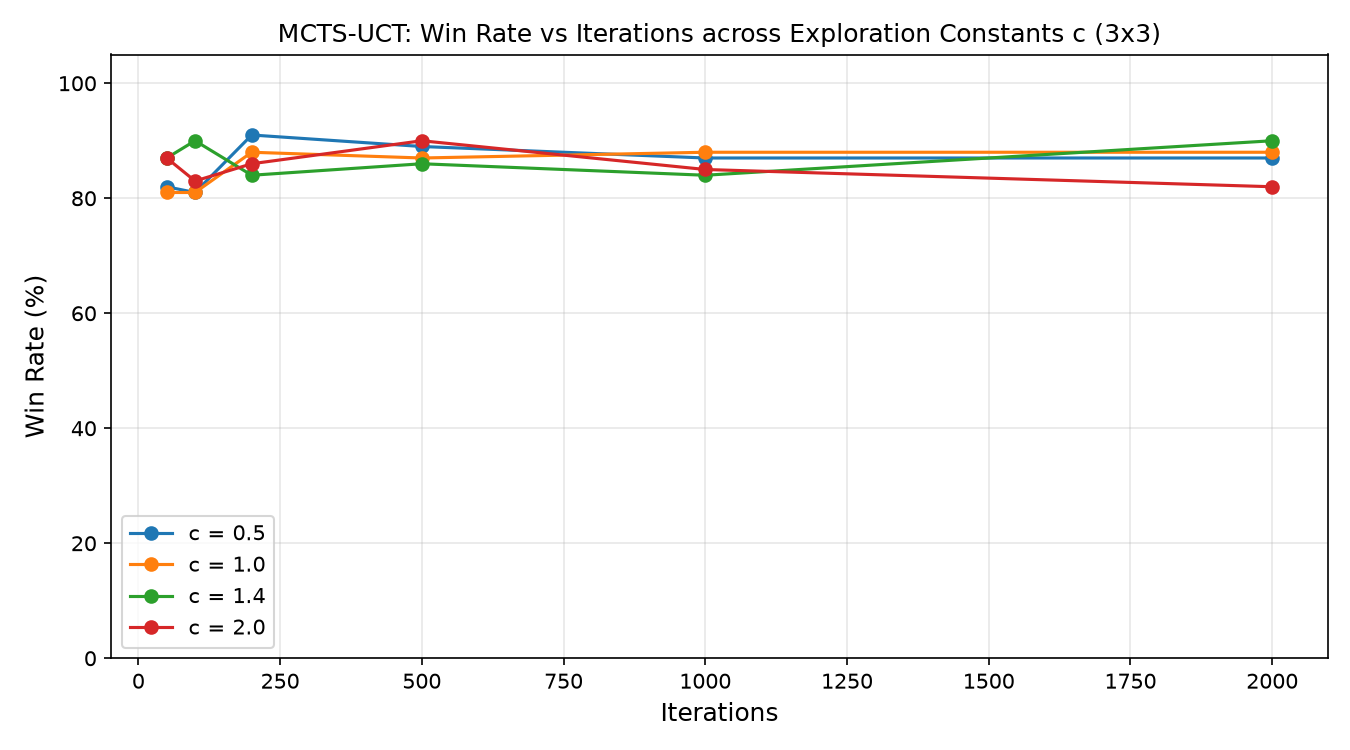
\includegraphics[width=0.95\linewidth]{../assets/figures/winrate_vs_iterations_3x3.png}
\caption{MCTS-UCT win rate vs iterations on $3\times 3$ (100 games/config).}
\label{fig:winrate_3x3}
\end{figure}

\begin{figure}[t]
\centering
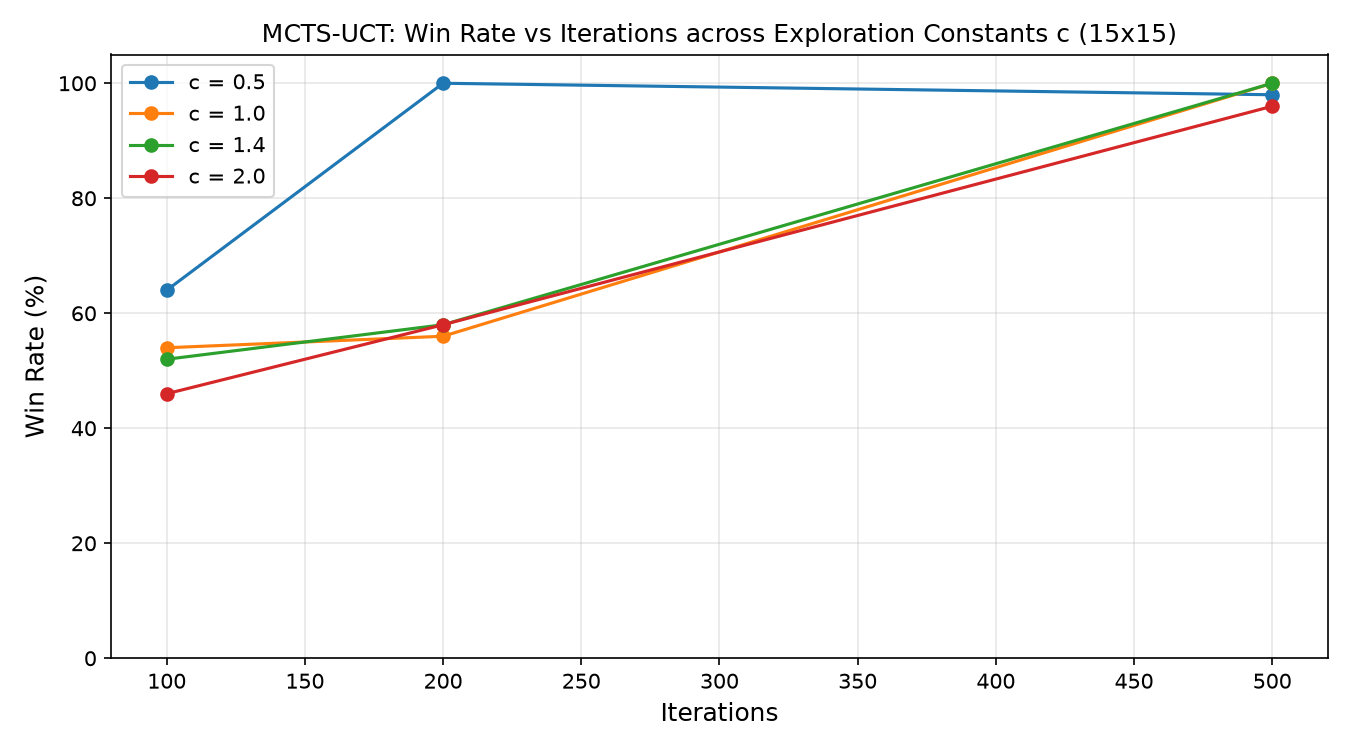
\includegraphics[width=0.95\linewidth]{../assets/figures/winrate_vs_iterations_15x15.png}
\caption{MCTS-UCT win rate vs iterations on $15\times 15$ (50 games/config).}
\label{fig:winrate_15x15}
\end{figure}

\subsection{Root Node Statistics ($W$, $N$, $W/N$)}
Table~\ref{tab:root_stats} shows root child statistics after $1000$ iterations ($c = 1.0$) on the $3\times 3$ test state ($X$ at $(1,1)$, $O$ at $(0,0)$) and the $15\times 15$ opening state. On $3\times 3$, UCT concentrates $545/1000$ visits on the two strongest moves $(0,1)$ and $(1,0)$. On $15\times 15$, because $30$-step random rollouts rarely terminate in the opening, $W/N$ values cluster tightly around $0.50$--$0.53$.

\begin{table}[t]
\centering
\caption{Root Node Statistics ($1000$ Iterations, $c = 1.0$)}
\label{tab:root_stats}
\begin{tabular}{@{}crrr|crrr@{}}
\toprule
\multicolumn{4}{c|}{$3\times 3$ Test State} & \multicolumn{4}{c}{$15\times 15$ Opening (Top 7)} \\
Move & $W$ & $N$ & $W/N$ & Move & $W$ & $N$ & $W/N$ \\
\midrule
(0, 1) & 242.5 & 299 & 0.811 & (5, 9) & 16.5 & 31 & 0.532 \\
(1, 0) & 195.0 & 246 & 0.793 & (10, 7) & 15.5 & 30 & 0.517 \\
(2, 0) & 87.0 & 121 & 0.719 & (5, 8) & 15.5 & 30 & 0.517 \\
(0, 2) & 80.0 & 112 & 0.714 & (10, 5) & 15.5 & 30 & 0.517 \\
(2, 1) & 56.0 & 83 & 0.675 & (4, 8) & 15.0 & 29 & 0.517 \\
(1, 2) & 50.5 & 77 & 0.656 & (5, 6) & 15.0 & 29 & 0.517 \\
(2, 2) & 39.0 & 62 & 0.629 & (8, 6) & 15.0 & 29 & 0.517 \\
\bottomrule
\end{tabular}
\end{table}

\subsection{Random Rollout vs Heuristic Rollout}
Table~\ref{tab:rollout} compares random and heuristic rollouts at $c = \sqrt{2}$. Heuristic rollout improves win rate by $+6.0\%$ on $3\times 3$ and $+16.0\%$ on $15\times 15$, while increasing per-move latency on $15\times 15$ by only $1.52\times$ ($3{,}647 \rightarrow 5{,}553$~ms).

\begin{table}[t]
\centering
\caption{Random Rollout vs Heuristic Rollout ($c = \sqrt{2}$)}
\label{tab:rollout}
\setlength{\tabcolsep}{4pt}
\begin{tabular}{@{}ccclrrr@{}}
\toprule
Board & Iters & Games & Rollout & W/D/L & Win Rate & ms/move \\
\midrule
$3\times 3$ & 500 & 100 & Random & 84/16/0 & 84.0\% & 52.2 \\
$3\times 3$ & 500 & 100 & Heuristic & 90/10/0 & \textbf{90.0\%} & 51.2 \\
\midrule
$15\times 15$ & 200 & 50 & Random & 38/0/12 & 76.0\% & 3,647 \\
$15\times 15$ & 200 & 50 & Heuristic & 46/0/4 & \textbf{92.0\%} & 5,553 \\
\bottomrule
\end{tabular}
\end{table}

\subsection{UCT Formula Variants and Progressive Bias}
Table~\ref{tab:uct_variants} and Fig.~\ref{fig:uct_variants} compare the four UCT ablations and Progressive Bias at $c = 1.0$. Removing $\ln$ (\texttt{no\_ln}) or both $\sqrt{\cdot}$ and $\ln$ (\texttt{linear}) degrades non-loss rate against optimal Alpha-Beta on $3\times 3$ from $96.0\%$ to $76.0\%$ and $65.0\%$, and drops $15\times 15$ win rate from $52.0\%$ to $34.0\%$. Conversely, Progressive Bias raises $15\times 15$ win rate at $150$ iterations from $52.0\%$ to \textbf{98.0\%} ($49/50$) while reducing average move latency ($2{,}709 \rightarrow 2{,}390$~ms).

\begin{table}[t]
\centering
\caption{UCT Variants and Progressive Bias ($c = 1.0$)}
\label{tab:uct_variants}
\scriptsize
\setlength{\tabcolsep}{2.5pt}
\begin{tabular}{@{}lccc@{}}
\toprule
Variant & $3\times 3$ vs AB (300) & $3\times 3$ vs Rand (200) & $15\times 15$ vs Rand (150) \\
 & Non-Loss (W/D/L) & Win / Non-Loss & Win (W/D/L) / ms \\
\midrule
Standard UCT & \textbf{96.0\%} (0/96/4) & 88.0\% / 98.0\% & 52.0\% (26/0/24) / 2,709 \\
No-sqrt & 95.0\% (0/95/5) & 84.0\% / 99.0\% & 44.0\% (22/0/28) / 2,629 \\
No-ln & 76.0\% (0/76/24) & 88.0\% / 97.0\% & 34.0\% (17/0/33) / 3,037 \\
Linear & 65.0\% (0/65/35) & 83.0\% / 93.0\% & 34.0\% (17/0/33) / 3,066 \\
\textbf{Prog.\ Bias} & 95.0\% (0/95/5) & \textbf{88.0\% / 100.0\%} & \textbf{98.0\%} (49/0/1) / \textbf{2,390} \\
\bottomrule
\end{tabular}
\end{table}

\begin{figure}[t]
\centering
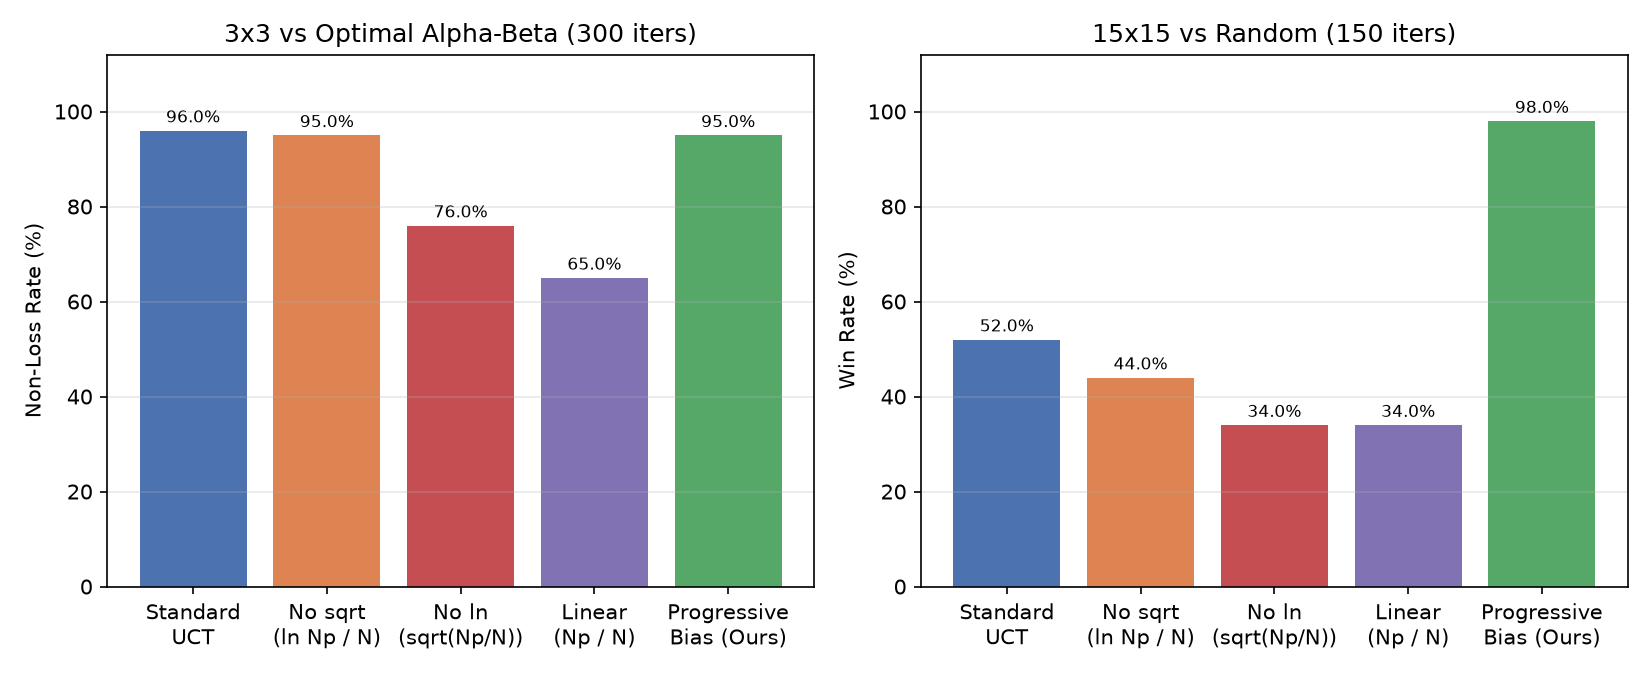
\includegraphics[width=0.98\linewidth]{../assets/figures/uct_variants_comparison.png}
\caption{Comparison of UCT formula ablations and Progressive Bias on $3\times 3$ (vs optimal Alpha-Beta) and $15\times 15$ (vs Random).}
\label{fig:uct_variants}
\end{figure}

\section{Discussion}

\textbf{RQ1 (Alpha-Beta Pruning Efficiency):} Alpha-Beta pruned $71.8\%$ of nodes at depth $4$ on $3\times 3$ and $88.0\%$ at depth $3$ on $15\times 15$. Pruning gains grow sharply with branching factor and depth, confirming why plain Minimax is unusable beyond depth $2$ on $15\times 15$ Gomoku.

\textbf{RQ2 (Effect of Exploration Constant $c$):} On $3\times 3$, all four values of $c$ reach $0$ losses against random play once $\text{iterations} \ge 500$. On $15\times 15$, the exploration--exploitation trade-off is pronounced at low budgets: $c = 0.5$ converges fastest ($64\%$ at $100$ iterations, $100\%$ at $200$ iterations), whereas larger $c$ values spend early budget exploring wide neighborhoods ($46$--$54\%$ at $100$ iterations). Once $\text{iterations} = 500$, all four constants converge to $96$--$100\%$, with $c = 1.0$ and $c = 1.4$ reaching $100\%$ ($50/50$). Thus, smaller $c$ ($0.5$) is preferable under tight budgets on large boards, while $c \in [1.0, 1.4]$ is optimal when sufficient budget is available.

\textbf{RQ3 (Never-Lose Property on $3\times 3$):} Against an optimal depth-$9$ Alpha-Beta player, MCTS still loses occasionally at low budgets ($11/50$ losses at $100$ iterations, $2/50$ at $500$ iterations for $c = 1.0$) because shallow trees miss forced forks. From $\text{iterations} \ge 1000$ onward, MCTS achieves $0$ losses out of $50$ games ($50$ draws) for both $c = 1.0$ and $c = 1.414$, empirically confirming the theoretical convergence of UCT on $3\times 3$ Tic-Tac-Toe.

\textbf{RQ4 (Heuristic Rollout vs Value Networks):} Replacing random rollout with a one-ply win/block heuristic improved win rate by $+6.0\%$ on $3\times 3$ and $+16.0\%$ on $15\times 15$ at only $1.52\times$ latency overhead thanks to in-place win/block checks without board cloning. Even a shallow tactical filter substantially reduces simulation noise on large boards. This mirrors the evolution from classical MCTS to AlphaGo/AlphaZero~\cite{silver2016}, where learned policy and value networks replace noisy rollouts with direct position evaluation and move priors.

\textbf{RQ5 (Selecting by $N$ vs $W/N$):} At the end of search, \texttt{get\_move()} selects \texttt{most\_visited\_child()} (highest $N$) rather than highest $W/N$. A rarely visited child can exhibit an inflated $W/N$ (e.g., $1.0$ from $1$--$2$ lucky rollouts) due to high sampling variance. Because UCT allocates visits asymptotically in proportion to arm quality, the most-visited child has both the tightest confidence bound and the lowest-variance value estimate.

\textbf{RQ6 (UCT Ablations \& Progressive Bias):} Removing $\ln$ (\texttt{no\_ln}) or both $\sqrt{\cdot}$ and $\ln$ (\texttt{linear}) causes the exploration term to grow polynomially with $N_{\mathrm{parent}}$, preventing UCT from concentrating visits on strong moves ($96.0\% \rightarrow 76.0\% / 65.0\%$ non-loss on $3\times 3$; $52.0\% \rightarrow 34.0\%$ win rate on $15\times 15$). Removing only $\sqrt{\cdot}$ (\texttt{no\_sqrt}) over-penalizes early visits and lowers $15\times 15$ win rate to $44.0\%$. Adding Progressive Bias ($H_i/(N_i+1)$) boosts $15\times 15$ win rate at $150$ iterations from $52.0\%$ to $98.0\%$ ($+46.0\%$) while reducing move latency ($2{,}709 \rightarrow 2{,}390$~ms) because games finish in fewer moves.

\textbf{Limitations:} (1) On $15\times 15$, capping rollouts at $30$ steps keeps runtime practical, but most early-game rollouts terminate undecided ($0.5$), flattening root $W/N$ values around $0.50$--$0.53$ (Table~\ref{tab:root_stats}); evaluating truncated rollouts with \texttt{evaluate()} would provide stronger signal. (2) \texttt{MCTSAgent} rebuilds the search tree from scratch on every move (no tree reuse), and \texttt{Board.get\_legal\_moves()} recomputes the radius-$2$ neighborhood from \texttt{move\_history} on every call. (3) Alpha-Beta depth $3$ on $15\times 15$ lacks move ordering and double-threat detection in \texttt{evaluate()}, making it vulnerable to multi-move forks.

\section{Conclusion}
We implemented and evaluated Minimax with Alpha-Beta pruning and MCTS-UCT on $3\times 3$ and $15\times 15$ Tic-Tac-Toe. Alpha-Beta prunes $71.8\%$ of nodes on $3\times 3$ (depth $4$) and $88.0\%$ on $15\times 15$ (depth $3$). On $3\times 3$, MCTS-UCT reaches $0$ losses against both random play ($\ge 500$ iterations) and optimal depth-$9$ Alpha-Beta ($\ge 1000$ iterations). On $15\times 15$, $c = 0.5$ converges fastest at low budgets ($100\%$ at $200$ iterations), while $c \in \{1.0, 1.4\}$ achieve $100\%$ ($50/50$) at $500$ iterations. Finally, a lightweight one-ply heuristic rollout boosts win rate by $+6.0\%$ on $3\times 3$ and $+16.0\%$ on $15\times 15$, demonstrating the core intuition behind neural value and policy networks in modern game AI.

\begin{thebibliography}{00}
\bibitem{auer2002} P. Auer, N. Cesa-Bianchi, and P. Fischer, ``Finite-time analysis of the multiarmed bandit problem,'' \emph{Machine Learning}, vol. 47, no. 2--3, pp. 235--256, 2002.
\bibitem{kocsis2006} L. Kocsis and C. Szepesv\'ari, ``Bandit based Monte-Carlo planning,'' in \emph{Proc. ECML}, 2006, pp. 282--293.
\bibitem{coulom2006} R. Coulom, ``Efficient selectivity and backup operators in Monte-Carlo tree search,'' in \emph{Proc. ICCG}, 2006, pp. 72--83.
\bibitem{silver2016} D. Silver et al., ``Mastering the game of Go with deep neural networks and tree search,'' \emph{Nature}, vol. 529, pp. 484--489, 2016.
\bibitem{chaslot2008} G. M. J.-B. Chaslot, M. H. M. Winands, H. J. van den Herik, J. W. H. M. Uiterwijk, and B. Bouzy, ``Progressive strategies for Monte-Carlo tree search,'' \emph{New Mathematics and Natural Computation}, vol. 4, no. 3, pp. 343--357, 2008.
\bibitem{russell2020} S. Russell and P. Norvig, \emph{Artificial Intelligence: A Modern Approach}, 4th ed. Pearson, 2020.
\end{thebibliography}

\end{document}
